\chapter{Collection of particles} \label{appendixinterf} 

In the section we are going to describe how to simulate collections of particles using \BornAgain\ \textit{i.e.} the way their spatial distributions and the distribution of shapes and their correlations can influence the output scattered intensity. The samples generated with \BornAgain\ are made of different material layers characterized by their thicknesses, refractive indices, and possible surface roughnesses. Except for the thickness, the other dimensions of the layers are infinite.\\ Particles can be embedded in or deposited on the top of any layers. Those particles are characterized by their shapes, refractive indices, their spatial distribution and concentration in the sample. When the particles are densely packed, the distance relative to each other becomes of the same order as the particles' sizes. The radiation scattered from these various particles are going to interfere together. The influence of the particles' shapes has been described in the previous section about form factors.

We do not consider any multiple scattering, polarisation (see Section...), nor layers' roughness (see Section...).\\ We are first going to give a short overview of the theory involved, mostly in order to define the terminology. For a more complete theoretical description, the user is referred to, for example, reference~\cite{ReLa09}. Then we are going to describe how the interference features have been implemented in \BornAgain\ and give some detailed examples.


%\MakeRemark{Terminology}{
%\\
%For collections of particles, the scattered intensity contains contributions from neighboring particles. This additional pattern can be called the structure factor, the interference function or even in crystallography, the lattice factor. In this manual, we use the term "interference function" or interferences.
%}

%%%%%%%%%%%%%%%%%%%%%%%%%%%%%%%%%%%%%%%%%%%%%%
%\section{Theory}

%Considering a set of $N$ particles labeled with index $i$, located at $\mathbf{R}_i$ and having shapes $S_i(\mathbf{r})$ ($S_i=0$ outside the particle and 1 inside), the scattered intensity per particle is given by:
%\begin{equation}
%  I(\mathbf{q}) = \frac{1}{N}\left\langle \left\lvert \sum_i F_i(q)e^{i \mathbf{q}\cdot \mathbf{R}_i}\right\rvert^{2} \right\rangle =\frac{1}{N}\left\langle \sum_i |F_i(\mathbf{q})|^2+\sum_{i \neq j} F_i(\mathbf{q}) F_j ^*(\mathbf{q})\exp(i\mathbf{q}\cdot (\mathbf{R}_i-\mathbf{R}_j)) \right\rangle, \label{eq:interfintensity}
%\end{equation}

%where $\langle\ldots\rangle$ denotes a spatial and temporal average, $\mathbf{q}$ is the wave vector (in reciprocal space) and $F_i$ is the form factor of particle $i$ evaluated using the Distorted Wave Born Approximation. 

%If only the statistical quantities of the system are known (particles' positions and sizes), the discrete sums in equation~\ref{eq:interfintensity} can be replaced by continuous integrals using some probability densities. For example, in two dimensions (which is the case for particles deposited on a surface), the probability per unit surface to find a particle of class $\alpha$ in $\mathbf{R}_{i}$ knowing that there is a particle of type $\beta$ in $\mathbf{R}_{j}$ can be written as  $\rho_S^2 g_{\alpha \beta}(R_{i,\alpha},R_{j,\beta})$ where $\rho_S$ is the number of particles  per unit surface and $g_{\alpha \beta}$ is the partial pair correlation function, which tends towards 1 as the distance between the particles increases.


%%%%%%%%%%%%%%%%%%%%%%%%%%%%%%%%%%%%%%%%
%\subsection{Size-distribution models}

%To proceed further, when the morphology and topology are not exactly known, some hypotheses need to be made since the correlation between the kinds of scatterers and their relative positions included in $g_{\alpha \beta}$ are difficult to estimate. Several options are available:

%\paragraph{Decoupling approximation (DA)} neglects all correlations. It supposes that the particles are positioned in a way that is completely independent on their kinds (shapes, sizes). Thus the kind of scattering objects and their positions are not correlated. This leads to the following expression of the scattered intensity:

%\begin{equation*}
%I(\mathbf{q})= |\langle F(\mathbf{q})\rangle |^2 S(\mathbf{q})+ \underbrace{\langle |F(\mathbf{q})|^2\rangle-|\langle F(\mathbf{q})\rangle |^2}_{\text{incoherent\, term}}
%\end{equation*}
%where $S(\mathbf{q})$ is the total interference function (\textit{i.e.} the Fourier transform of the particle position autocorrelation function).\\
%In concentrated systems, DA breaks down because of correlations. One solution is to reintroduce some correlations between particles sizes and distributions (using for example the Size spacing correlation approximation described below). 

 
%\paragraph{Local monodisperse approximation (LMA)} partially accounts for some coupling between the positions and the kinds of the particles \cite{Pede94}. 
% It requires a subdivision of the layers of particles into monodisperse domains. The contributions of these subdomains are then  incoherently summed up and weighted by the size-shape probabilities.\\ In this approximation, a particle is supposed to be surrounded by particles of the same size and shape, within the coherence length of the input beam. The scattered intensity is expressed as
%\begin{equation*}
%I(\mathbf{q})= \langle |F(\mathbf{q})|^2   S(\mathbf{q}) \rangle 
%\end{equation*}
%One has to remember that in most cases, this approximation corresponds to an unphysical description of the investigated systems. \\ 

%DA and LMA separate the contributions of the form factors and of the interference function. For disordered systems DA and LMA give the same result as the scattering vector gets larger \textit{i.e.} the scattered intensity is dominated by the contribution of the form factor.

%\paragraph{Size spacing correlation approximation (SSCA)} introduces correlations between polydisperse particles and is derived from the paracrystal model (see description below and \cite{LeLa04}).

%%%%%%%%%%%%%%%%%%%%%%%%%%%%%%%%%%%%%%%%
\subsection{Layout of particles}\label{sec:partlayout}

\ImportantPoint{Remark:}{ The particles are positioned in the same vertical layer.}

%\subsubsection{The uncorrelated or disordered lattice}
%For very diluted distributions of particles, the particles are too far apart from each other to lead to any interference between the waves scattered by each of them. In this case the interference function is equal to 1. The scattered intensity is then entirely determined by the form factors of the particles distributed in the sample.

%\subsubsection{The regular  lattice}
%The particles are positioned at regular intervals generating a layout characterised by its base vectors $\mathbf{a}$ and $\mathbf{b}$ (in direct space) and the angle between these two vectors.
%This lattice can be two or one-dimensional depending on the characteristics of the particles. For example when they are infinitely long, the implementation can be simplified and reduced to a "pseudo" 1D system.

%\subsubsection{The ideal paracrystal} 
%A paracrystal, whose notion  was developed by Hosemann\cite{Hos51}, allows fluctuations of the lengths and orientations of lattice vectors. Paracrystals can be defined as distorted crystals in which the crystalline order has not disappeared and for which the behavior of the interference functions  at small angles is coherent.
%It is a transition between the regular lattice and the disordered state.\\


%For example, in one dimension, a paracrystal is generated using the following method. First we place a particle at the origin. The second particle is put at a distance $x$ with a density probability $p(x)$ that is peaked at a mean value $D$: $\int_{-\infty} ^{\infty}p(x)dx=1$ and $\int_{-\infty}^{\infty}xp(x)dx=D$. The third one is added at a distance $y$ from the second site using the same rule with a density probability $p_2(y)= \int_{-\infty}^{\infty}p(x)p(y-x)dx=p\otimes p(y)$.\\ With such a method, the pair correlation function $g(x)$ is built step by step. Its expression and the one of its Fourier transform, which is the interference function are 
%\begin{equation*}
%g(x)=\delta(x)+ p(x)+ p(x)\otimes p(x)+\ldots + p(-x)+\ldots \: \mathrm{and}\:\, S(q)=\Re\left(\dfrac{1+P(q)}{1-P(q)}\right),
%\end{equation*}
% where $P(q)$ is the Fourier transform of the density probability $p(x)$.\\


%In two dimensions, the paracrystal is constructed on a pseudo-regular lattice with base vectors $\mathbf{a}$ and $\mathbf{b}$ using the following conditions for the densities of probabilities:\\ $\int p_{\mathbf{a}}(\mathbf{r})d^2\mathbf{r}=\int p_{\mathbf{b}}(\mathbf{r})d^2\mathbf{r}=1$, $\int \mathbf{a} p_{\mathbf{a}}(\mathbf{r})d^2\mathbf{r}=\mathbf{a}$, $\int \mathbf{b} p_{\mathbf{b}}(\mathbf{r})d^2\mathbf{r}=\mathbf{b}$.\\
%In the ideal case the two axes are decoupled and each unit cell should retain a parallelogram shape. The interference function is given by $S(q_{\parallel})=\prod_{k=a,b}\Re\left(\dfrac{1+P_k(q_{\parallel})}{1-P_k(q_{\parallel})} \right)$ with $P_k$ the Fourier transform of $p_k$, $k=a, b$.

\subsubsection{Probability distributions} \label{baftd} 
The scattering by an ordered lattice gives rise to a series of Bragg peaks situated at the nodes of the reciprocal lattice. Any divergence from the ideal crystalline case modifies the output spectrum by, for example, widening or attenuating the Bragg peaks. The influence of these "defects" can be accounted for  in direct space using correlation functions or by truncating the lattice or, in reciprocal space with structure factors or interference functions by convoluting the scattered pics with a function which could reproduce the experimental shapes.\\ The later option has been implemented in \BornAgain. The Fourier transforms of the probability distribution functions in 1 and 2D are listed in Table~\ref{table:pdf}. 

\begin{table}
\centering
\begin{tabular}{ccc}
\hline 
Function & One dimension & Two dimensions\\
\hline 
Cauchy & $(1+q^2\omega^2)^{-3/2}$ & $(1 + q_x^2 cl_x^2 + q_y^2 cl_y^2)^{-3/2}$ \\
Gauss & $\dfrac{1}{2}\exp(-\dfrac{q^2\omega^2}{4})$ & $\frac{1}{2}\exp\left(-\dfrac{q_x^2 cl_x^2+ q_y^2cl_y^2}{4}\right)$ \\
Voigt & $\dfrac{\eta}{2} \exp\left(-\dfrac{q^2\omega^2}{4}\right) + \dfrac{1 - \eta}{(1 + q^2\omega^2)^{3/2}}$ & $\dfrac{\eta}{2} \exp\left(-\dfrac{q_x^2 cl_x^2+ q_y^2cl_y^2}{4}\right)+ \dfrac{1 - \eta}{(1 + q_x^2 cl_x^2+ q_y^2cl_y^2)^{3/2}}$ \\
\hline
\end{tabular}
\caption{List of probability distribution functions in reciprocal space. $\omega$, $cl$ stand for coherence lengths (the index refers to the axis) and  $\eta$ is a weighting coefficient.}
\label{table:pdf}
\end{table}

The Cauchy distribution corresponds to $\exp(-r)$ in real space and the Voigt one  is a linear combination of the Gaussian and Cauchy probability distribution functions.

%%%%%%%%%%%%%%%%%%%%%%%%%%%%%%%%%%%%%%%%
\section{Implementation in \BornAgain}
\subsection{Size-distribution models}
The decoupling approximation, local monodisperse approximation and size spacing correlation approximation can be used in \BornAgain.
The selection is made using\\ \Code{ILayout.setApproximation(EInterferenceFunction approximation)} when defining the characteristics of the way particles and interference functions are embedded in a layer or by adding multiple ParticleLayout objects in a single layer (for the Local Monodisperse Approximation).  For example,
\begin{lstlisting}[language=python, style=eclipseboxed,numbers=none,nolol]
    particle_layout = ParticleLayout()
   ....
# interference approx chosen between: DA (default) and SSCA
    particle_layout.setApproximation(ILayout.DA)
\end{lstlisting}

The users can refer to Script~\ref{lst:2dlatticeinterf} for a more detailed implementation. By default, the decoupled approximation (DA) is used.

%%%%%%%%%%%%%%%%%%%%%%%%%%%%%%%%%%%%%%%%
\subsection{Probability distribution functions}\label{baftd}
The expressions in the reciprocal space are given in Table~\ref{table:pdf}.

\paragraph{One dimension}
\begin{itemize}
\item \Code{FTDistribution1DCauchy($\omega$)},
\item \Code{FTDistribution1DGauss($\omega$)},
\item \Code{FTDistribution1DVoigt($\omega, \eta$)}.
\end{itemize}
where $\omega$ is the coherence length and $\eta$ is a weighting factor.

\paragraph{Two dimensions}

\begin{itemize}
\item \Code{FTDistribution2DCauchy($cl_x$, $cl_y$)},
\item \Code{FTDistribution2DGauss($cl_x$, $cl_y$)},
\item \Code{FTDistribution2DVoigt($cl_x$, $cl_y$)}
\end{itemize}
where $cl_{x,y}$ are the coherence lengths in the $x$ or $y$ direction, respectively.

These functions can be used with all interference functions except the case without any interference and the one dimensional paracrystal, for which only the Gaussian case has already been implemented.
%%%%%%%%%%%%%%%%%%%%%%%%%%%%%%%%%%%%%%%%
\subsection{Interferences}
The interference function is specified when building the sample. It is linked with the particles (shape, material). Examples of implementation are given at the end of each description.

\paragraph{Syntax:}
 \Code{particle\_layout.addInterferenceFunction(interference\_function)},\\ where \Code{particle\_layout} holds the information about the different shapes and their proportions for a given layer of particles, and \Code{interference\_function}  is one of the following expressions:
\begin{itemize}
\item \Code{InterferenceFunctionNone()}
\item \Code{InterferenceFunction1DLattice(lattice\_parameters)}
\item \Code{InterferenceFunction1DParaCrystal(peak\_distance, width,corr\_length)}
\item \Code{InterferenceFunction2DLattice(lattice\_parameters)}
\item \Code{InterferenceFunction2DParaCrystal(length\_1, length\_2, $\alpha$\_lattice, $\xi$, \\ corr\_length)}
\end{itemize}
We are now going to describe these interference functions.\\


\ImportantPoint{Remark:}{\Code{InterferenceFunction1DLattice} can only be used for particles which are infinitely long in one direction of the sample's surface like for example a rectangular grating.}

\newpage
%%%%%%%%%%%%%%%%%%%%%%%%%%%%%%%%%%%%%%%%%%
\subsubsection{\ding{253} \Code{InterferenceFunctionNone()}} \label{paragraphnointerf}
The particles are placed randomly in the dilute limit and are considered as individual, non-interacting scatterers. The scattered intensity is function of the form factors only. 

\paragraph{Example} The sample is made of a substrate on which are deposited half-spheres. Script~\ref{lst:nointerf} details the commands necessary to generate it. Figure~\ref{fig:nointerf} shows an example of output intensity: Script~\ref{lst:nointerf}  + detector + input beam. The full script UMInterferencesNone.py can be found in /Examples/python/UsrManual. 


\begin{figure}[h]
\begin{center}
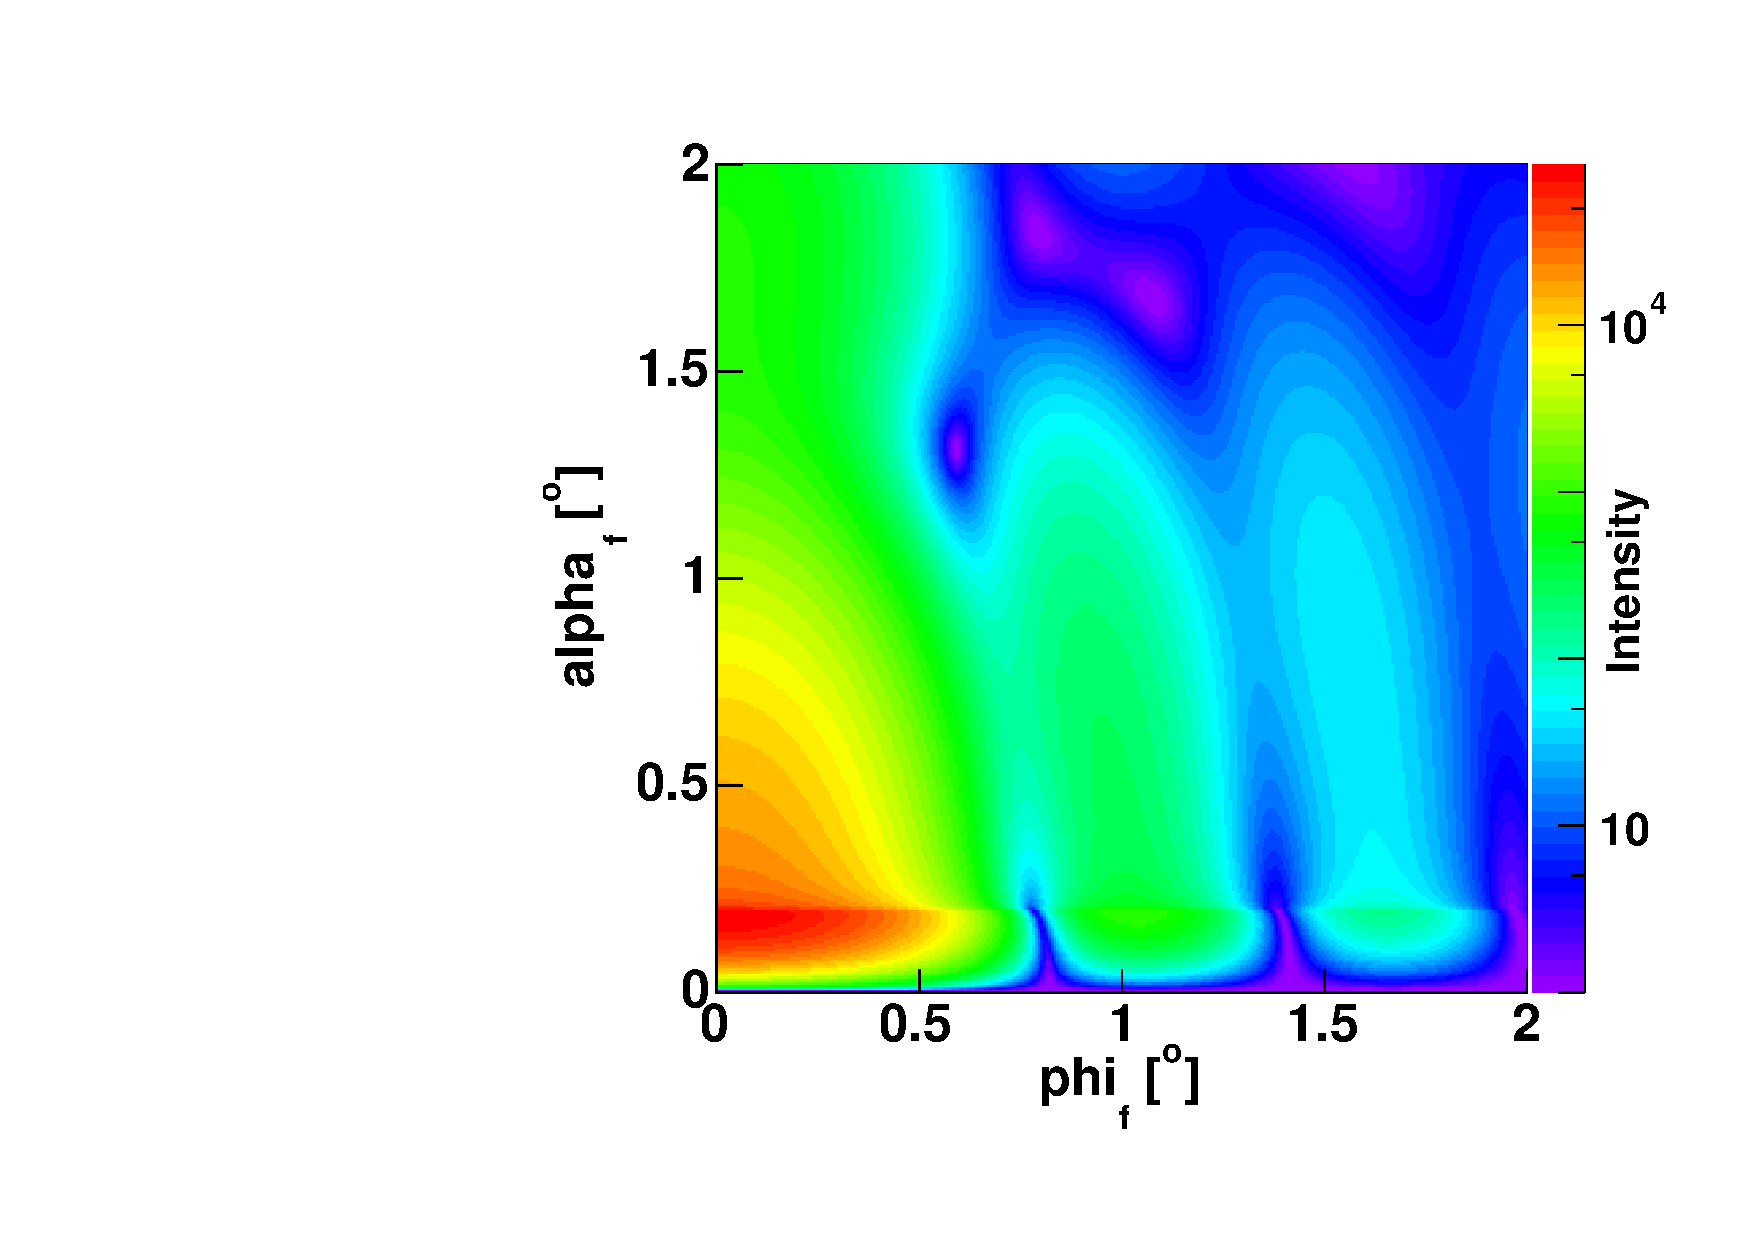
\includegraphics[width=0.5\textwidth]{Figures/HSphere_NoInterf}
\end{center}
\caption{Output intensity scattered from a sample made of half-spheres with no interference between them.}
\label{fig:nointerf}
\end{figure}

\FloatBarrier
\newpage

\begin{lstlisting}[language=python, style=eclipseboxed,numbers=none,nolol,caption={\Code{Python} script to simulate a sample made of half-spheres deposited on a substrate layer without any interference. The part specific to the interferences is marked in red italic font.},label={lst:nointerf}]
def get_sample():
    """
    Build and return the sample representing particles with no interference
    """
    # defining materials
    m_ambience = HomogeneousMaterial("Air", 0.0, 0.0)
    m_substrate = HomogeneousMaterial("Substrate", 6e-6, 2e-8)
    m_particle = HomogeneousMaterial("Particle", 6e-4, 2e-8)
    # collection of particles
    sphere_ff = FormFactorTruncatedSphere(5*nanometer, 5*nanometer)
    sphere = Particle(m_particle, sphere_ff)
    particle_layout = ParticleLayout()
    particle_layout.addParticle(sphere, 0.0, 1.0)
    |interference = InterferenceFunctionNone()| 
    |particle_layout.addInterferenceFunction(interference)|
    # assembling the sample
    air_layer = Layer(m_ambience)
    air_layer.addLayout(particle_layout)
    substrate_layer = Layer(m_substrate, 0)

    multi_layer = MultiLayer()
    multi_layer.addLayer(air_layer)
    multi_layer.addLayer(substrate_layer)
    return multi_layer
\end{lstlisting}

\newpage{\cleardoublepage}
%%%%%%%%%%%%%%%%%%%%%%%%%%%%%%%%%%%%%%%%%%
\subsubsection{\ding{253}  \Code{InterferenceFunction1DLattice(lattice\_parameters)}} \label{paragraph1dlatt}
where  \Code{lattice\_parameters}=(lattice\_length, $\xi$) with lattice\_length is the lattice constant and $\xi$ the angle in radian between the lattice unit vector and the $\mathbf{x}$-axis of the "GISAS experiment" referential as shown in fig.~\ref{fig:1dgrating}.

\begin{figure}[h]
\begin{center}
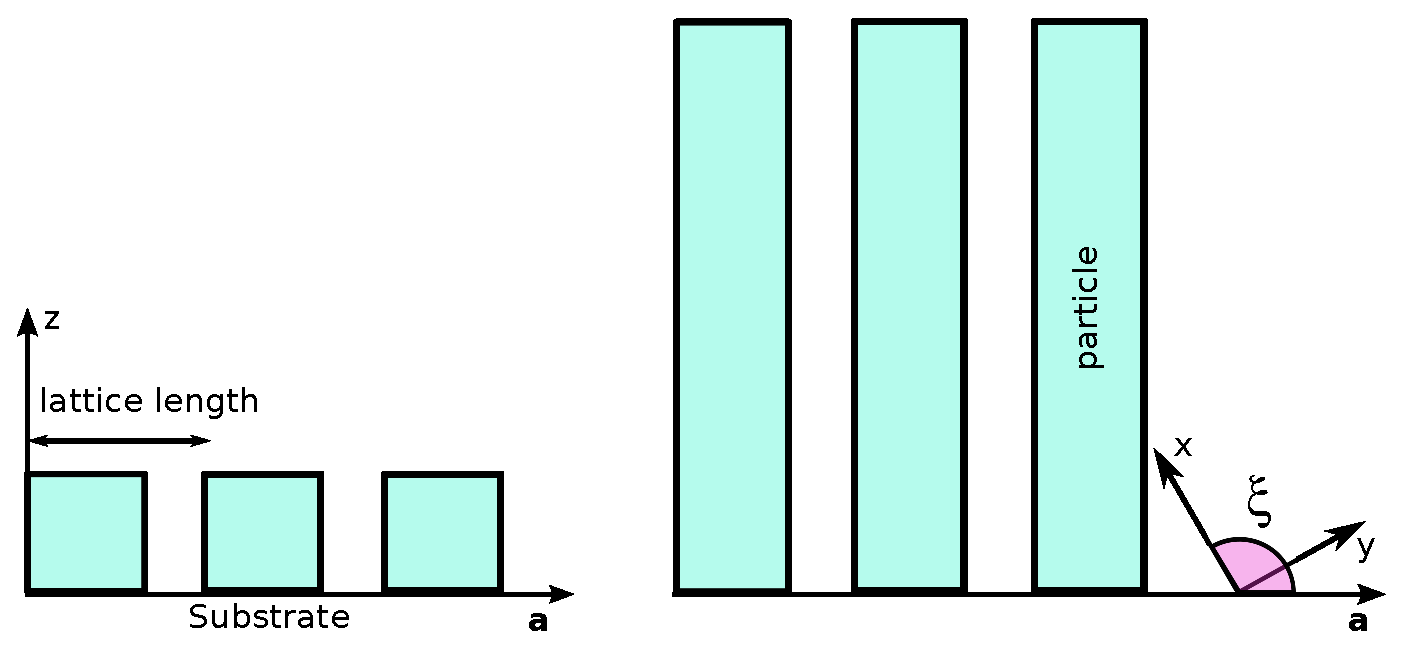
\includegraphics[width=0.75\textwidth]{Figures/1DGrating}
\end{center}
\caption{Schematic representation of a 1D lattice (side and top views). Such a lattice is characterized by a lattice length and the angle $\xi$.}
\label{fig:1dgrating}
\end{figure}

\ImportantPoint{Remark:}{By default the long axis of the particles in this 1D lattice is along the beam axis: $\xi=90^{\circ}$.}

\vspace{12pt}
A probability distribution function \Code{pdf} has to be chosen from the list in section~\ref{baftd} in order to apply some  modifications to the scattering peaks. This function is implemented using \Code{setProbabilityDistributions(pdf)}. 

\paragraph{Example:} Instead of giving a full script to generate the scattered intensity plot, we are focusing on how to build a sample using \Code{InterferenceFunction1DLattice} as the interference function in \BornAgain .\\ Script~\ref{lst:1dlattinterf} details this procedure in \Code{Python}. As mentioned previously, this interference function can only be used with infinitely wide or long particles.\\ Here the sample is made of infinitely long boxes deposited on a substrate (these particles are characterized by their widths and heights). They are also rotated by $90^{\circ}$  in the sample surface in order to have their long axis perpendicular to the input beam, along the $x$-axis.\\
 The lattice parameters (the lattice lengths and angle between the lattice main axis and the $x$-axis) are specified using \Code{Lattice1DIFParameters()} and are then used as input parameters of the interference function.

\newpage
\begin{lstlisting}[language=python, style=eclipseboxed,numbers=none,nolol,caption={\Code{Python} script to generate a sample made of infinitely lonx boxes deposited on a substrate layer with the 1DLatticeInterference function. The part specific to the interferences is marked in red italic font.},label={lst:1dlattinterf}]
def get_sample():
    """
    Build and return the sample with 1DLatticeInterference function
    """
    # defining materials
    m_air = HomogeneousMaterial("Air", 0.0, 0.0)
    m_substrate = HomogeneousMaterial("Substrate", 6e-6, 2e-8)
    m_particle = HomogeneousMaterial("Particle", 6e-4, 2e-8)

    # collection of particles
    ff = FormFactorInfLongBox(10.*nanometer, 15.0*nanometer)
    box = Particle(m_particle, ff)
    particle_layout = ParticleLayout()
    transform = Transform3D.createRotateZ(90.0*degree)
    particle_layout.addParticle(box, transform)

    # lattice parameters
    |lattice_params = Lattice1DIFParameters()|
    |lattice_params.m_length = 30.0*nanometer|
    |lattice_params.m_xi = 0.0*degree|

    # interference function
    |interference = InterferenceFunction1DLattice(lattice_params)|
    |pdf = FTDistribution1DCauchy(200./2./M_PI*nanometer)|
    |interference.setProbabilityDistribution(pdf)|
    |particle_decoration.addInterferenceFunction(interference)|

    # air layer with particles and substrate form multi layer
    air_layer = Layer(m_air)
    air_layer.setDecoration(particle_decoration)
    substrate_layer = Layer(m_substrate, 0)

    multi_layer = MultiLayer()
    multi_layer.addLayer(air_layer)
    multi_layer.addLayer(substrate_layer)
    return multi_layer
\end{lstlisting} 

\newpage{\cleardoublepage}
%%%%%%%%%%%%%%%%%%%%%%%%%%%%%%%%%%%%%%%%%%
\subsubsection{\ding{253} \Code{InterferenceFunction1DParaCrystal(peak\_distance, width, corr\_length)}}  \label{paragraph1dpara}
\begin{itemize}
\item[where] \Code{peak\_distance} is the average distance to the first neighbor peak, 
\item[]\Code{width} is the width parameter of the probability distribution,
\item[] \Code{corr\_length} is the correlation length (equal to 0 by default).
\end{itemize}

For this particular interference function, the implemented probability distribution function is Gaussian:

\begin{equation*}
p(x)=\frac{1}{\omega \sqrt{2\pi}} \exp\left(-\dfrac{(x-D)^2}{\omega^2}\right),\qquad P(q_{\parallel})=\exp\left(-\frac{q_{\parallel}^2 \omega^2}{2}\right)\exp(iq_{\parallel}D)
\end{equation*}
where $\omega\equiv$\Code{width}, $D\equiv$ \Code{peak\_distance}, and $q_{\parallel}=\sqrt{\Re^2(q_x) + \Re^2(q_y)}$ (see fig.~\ref{fig:1dpara}).

\begin{figure}[h]
\begin{center}
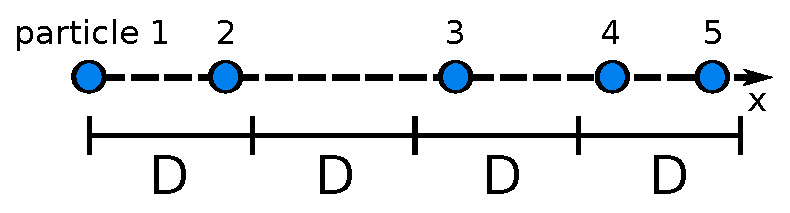
\includegraphics[width=0.5\textwidth]{Figures/1Dparacrystal}
\end{center}
\caption{Schematic representation of a 1D paracrystal in real space (side view). $D$ is the average spacing between the particles.}
\label{fig:1dpara}
\end{figure}

Using the procedure described in Section~\ref{sec:partlayout}, the interference function of a one-dimensional paracrystal is given by

\begin{align*}
S_{\mathrm{1DParaCrystal}}(q_{\parallel}) &=\Re \left(\frac{1+\Phi(q_{\parallel}) }{1 - \Phi(q_{\parallel})} \right), \\
\mathrm{where}\quad \Phi(q_{\parallel}) &= \left\{
\begin{array}{c l}     
    P(q_{\parallel}) & \mathrm{if\ \Code{corr\_length}}=0\\
    P(q_{\parallel})\exp\left(-\frac{D}{\mathrm{\Code{corr\_length}}}\right) & \mathrm{otherwise}
\end{array}\right.&
\end{align*}
%$\kappa$  is the size-distance coupling constant (equal to 0 by default) for Size Spacing Correlation Approximation

\paragraph{Example}
To illustrate the 1D paracrystal interference function, we use the same sample as in the case without interference: half-spheres deposited on a substrate.

\begin{lstlisting}[language=python, style=eclipseboxed,numbers=none,nolol,caption={\Code{Python} script to define the 1D paracrystal interference function between half-spheres, where \Code{trsphere} is of type \Code{Particle}.},label={lst:1dpara}]
    particle_layout = ParticleLayout()
    particle_layout.addParticle(trsphere, 0.0, 1.0)
    interference = InterferenceFunction1DParaCrystal(25.0*nanometer, 7*nanometer, 1e3*nanometer)
    particle_layout.addInterferenceFunction(interference)
\end{lstlisting}

\begin{figure}[h]
\begin{center}
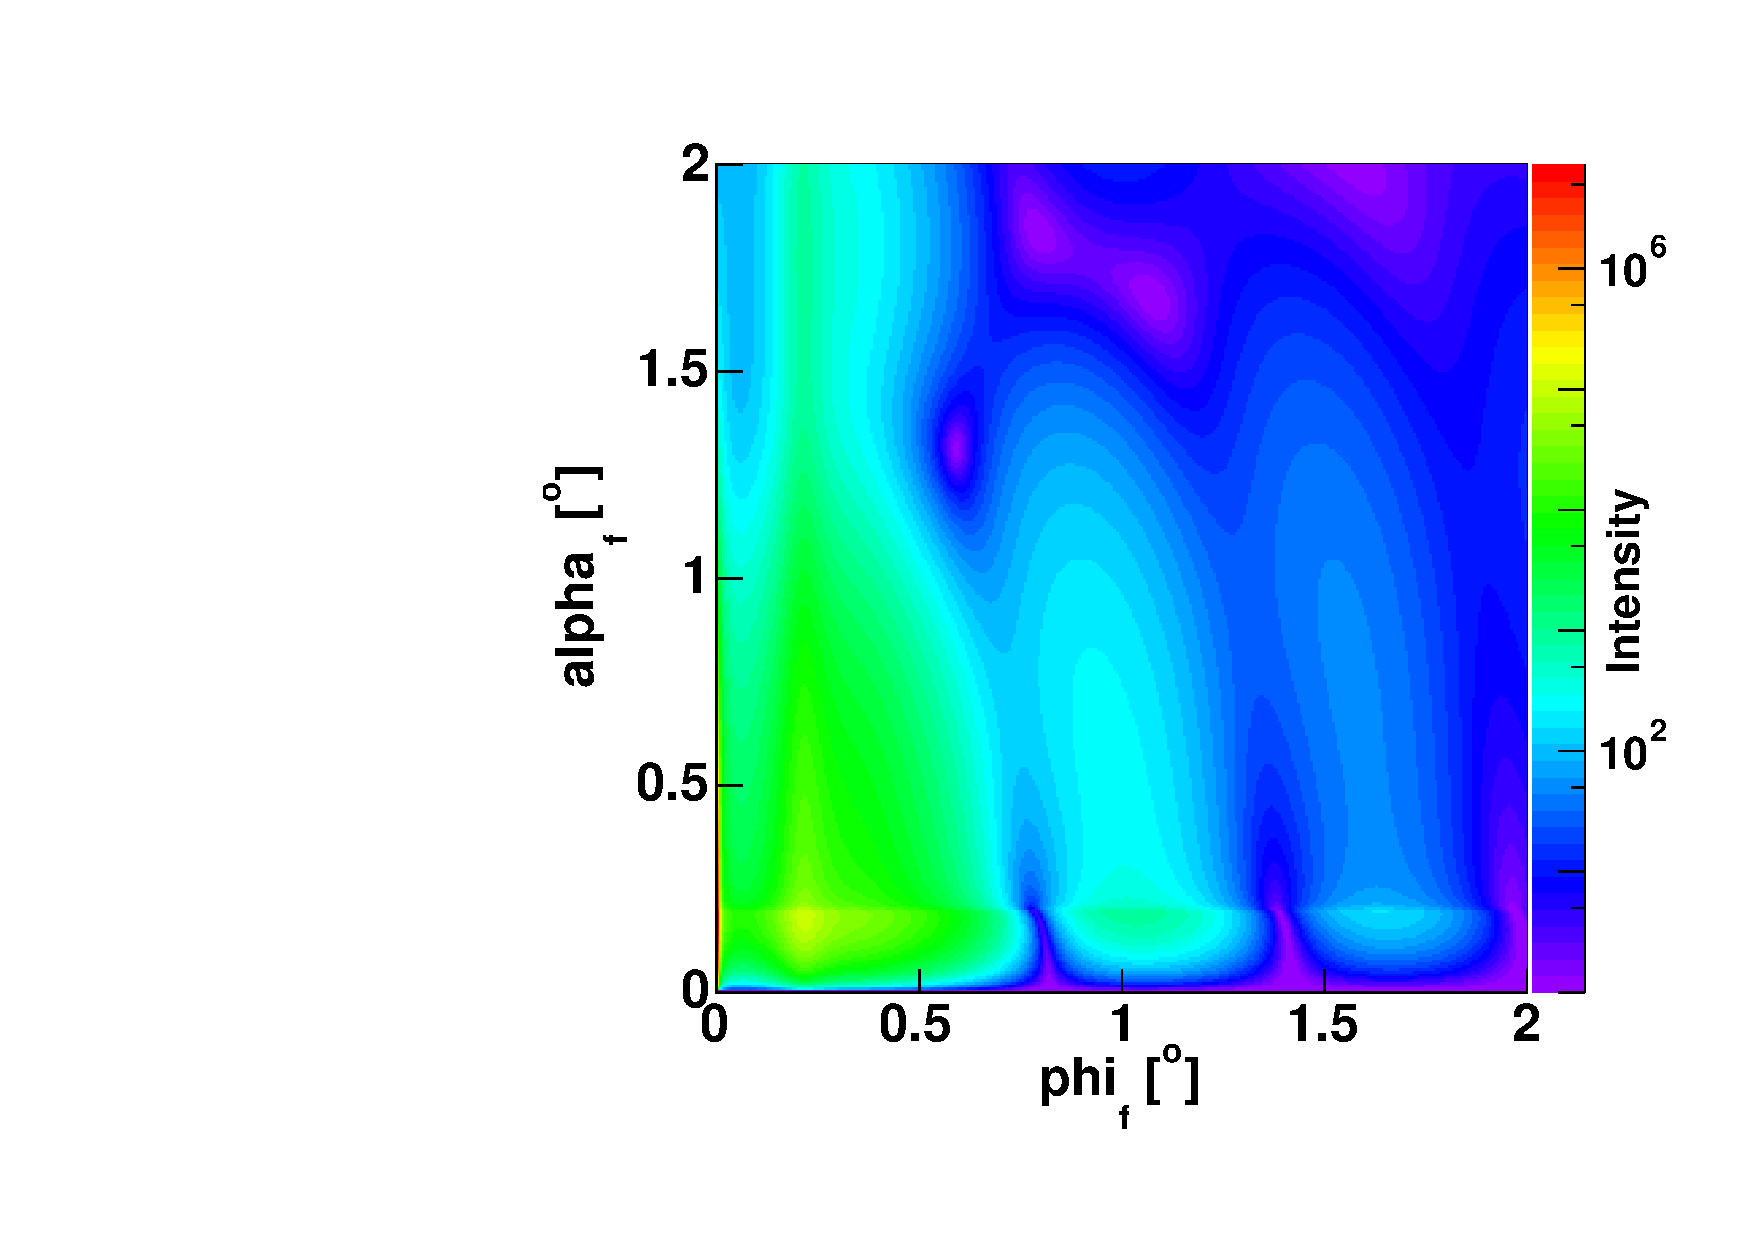
\includegraphics[width=0.5\textwidth]{Figures/HSphere_1DDL}
\end{center}
\caption{Output intensity scattered from a sample made of half-spheres with 1Dparacrystal interference between them. This figure has been generated using Script~\ref{lst:1dpara} for the interference function. The full script UMInterferences1DParaCrystal.py can be found at /Examples/python/UserManual.}
\label{fig:1ddl}
\end{figure}

\FloatBarrier

\newpage{\cleardoublepage}
%%%%%%%%%%%%%%%%%%%%%%%%%%%%%%%%%%%%%%
\subsubsection{\ding{253}  \Code{InterferenceFunction2DLattice(lattice\_parameters)}} \label{paragraph2dlatt}
where \Code{lattice\_parameters} corresponds to ($L_1$, $L_2$, $\alpha$, $\xi$)  (see illustration in figure~\ref{fig:2dlattice}) with 
\begin{itemize}
\item[]$L_1$, $L_2$ the lengths of the lattice cell, 
\item[]$\alpha$ the angle between the lattice basis vectors $\mathbf{a}, \mathbf{b}$ in direct space,
\item[] $\xi$ is the angle defining the lattice orientation (set to $0$ by default); it is taken as the angle between the $\mathbf{a}$ vector of the lattice basis and the $\mathbf{x}$ axis of the "GISAS experiment" referential (as shown in figure~\ref{fig:multil3d}).
\end{itemize}

\begin{figure}[h]
\begin{center}
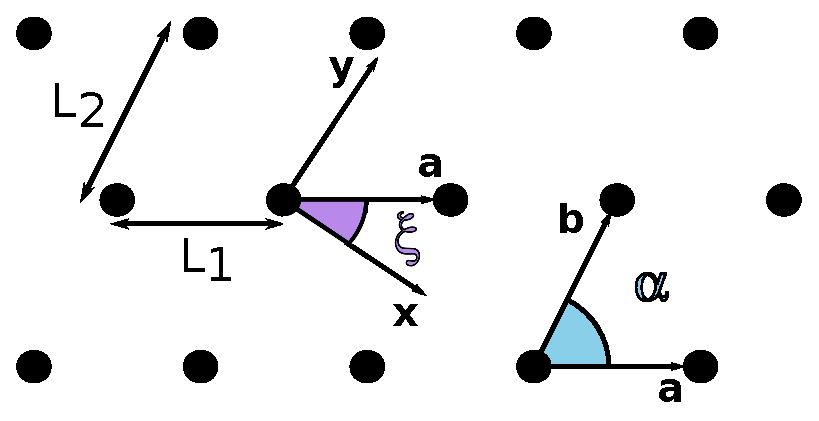
\includegraphics[width=0.5\textwidth]{Figures/2Dlattice.eps}
\end{center}
\caption{Schematic representation of a 2D lattice (top view). Such a lattice is characterized by lattice lengths $L_1$, $L_2$ and angles $\alpha$ and $\xi$.}
\label{fig:2dlattice}
\end{figure}

Like for the one-dimensional case, a probability distribution function \Code{pdf} has to be defined. One can choose between those listed in section \ref{baftd}. This function is implemented using \Code{setProbabilityDistributions(pdf)}.% Once defined the interference function is multiplied by a prefactor equal to $2\pi cl_x cl_y$, where $cl_x$, $cl_y$ are the correlation lengths in the $x-$ and $y-$directions.

\paragraph{Example} The sample used to run the simulation is made of half-spheres deposited on a substrate. The interference function is "2Dlattice" and the particles are located at the nodes of a square lattice with $L_1=L_2=20$~nm, $\mathbf{a}\equiv \mathbf{b}$ and the probability distribution function is Gaussian. We also use the Local Monodisperse Approximation. 

\begin{lstlisting}[language=python, style=eclipseboxed,numbers=none,nolol,caption={\Code{Python} script to define a 2DLattice interference function between hemi-spherical particles as well as the Decoupling Approximation in \Code{getSimulation()}.  The part specific to the interferences is marked in red italic font.},label={lst:2dlatticeinterf}]
    # lattice parameters
    |lattice_params = Lattice2DIFParameters()|
    |lattice_params.m_length_1 = 20.0*nanometer|
    |lattice_params.m_length_2 = 20.0*nanometer|
    |lattice_params.m_angle = 90.0*degree|
    |lattice_params.m_xi = 0.0*degree|

    #collection of particles
    sphere_ff = FormFactorTruncatedSphere(5*nanometer, 5*nanometer)
    sphere = Particle(m_particle, sphere_ff)
    |interference = InterferenceFunction2DLattice(lattice_params)|
    |pdf = FTDistribution2DGauss(200.0*nanometer/2.0/M_PI, 75.0*nanometer/2.0/M_PI)|
    |interference.setProbabilityDistribution(pdf)|
    particle_layout = ParticleLayout()
    particle_layout.addParticle(sphere, 0.0, 1.0)
    |particle_layout.addInterferenceFunction(interference)|

    # interference approx chosen between: DA (default) and SSCA
    |particle_layout.setApproximation(ILayout.DA)|
\end{lstlisting}
 
\begin{lstlisting}[language=python, style=eclipseboxed,numbers=none,nolol]
def get_simulation():
    """
    Create and return GISAXS simulation with beam and detector
    """
    simulation = Simulation()
    simulation.setDetectorParameters(100, 0.0*degree, 2.0*degree, 100, 0.0*degree, 2.0*degree)
    simulation.setBeamParameters(1.0*angstrom, 0.2*degree, 0.0*degree)
    return simulation
\end{lstlisting}


\begin{figure}[h]
\begin{center}
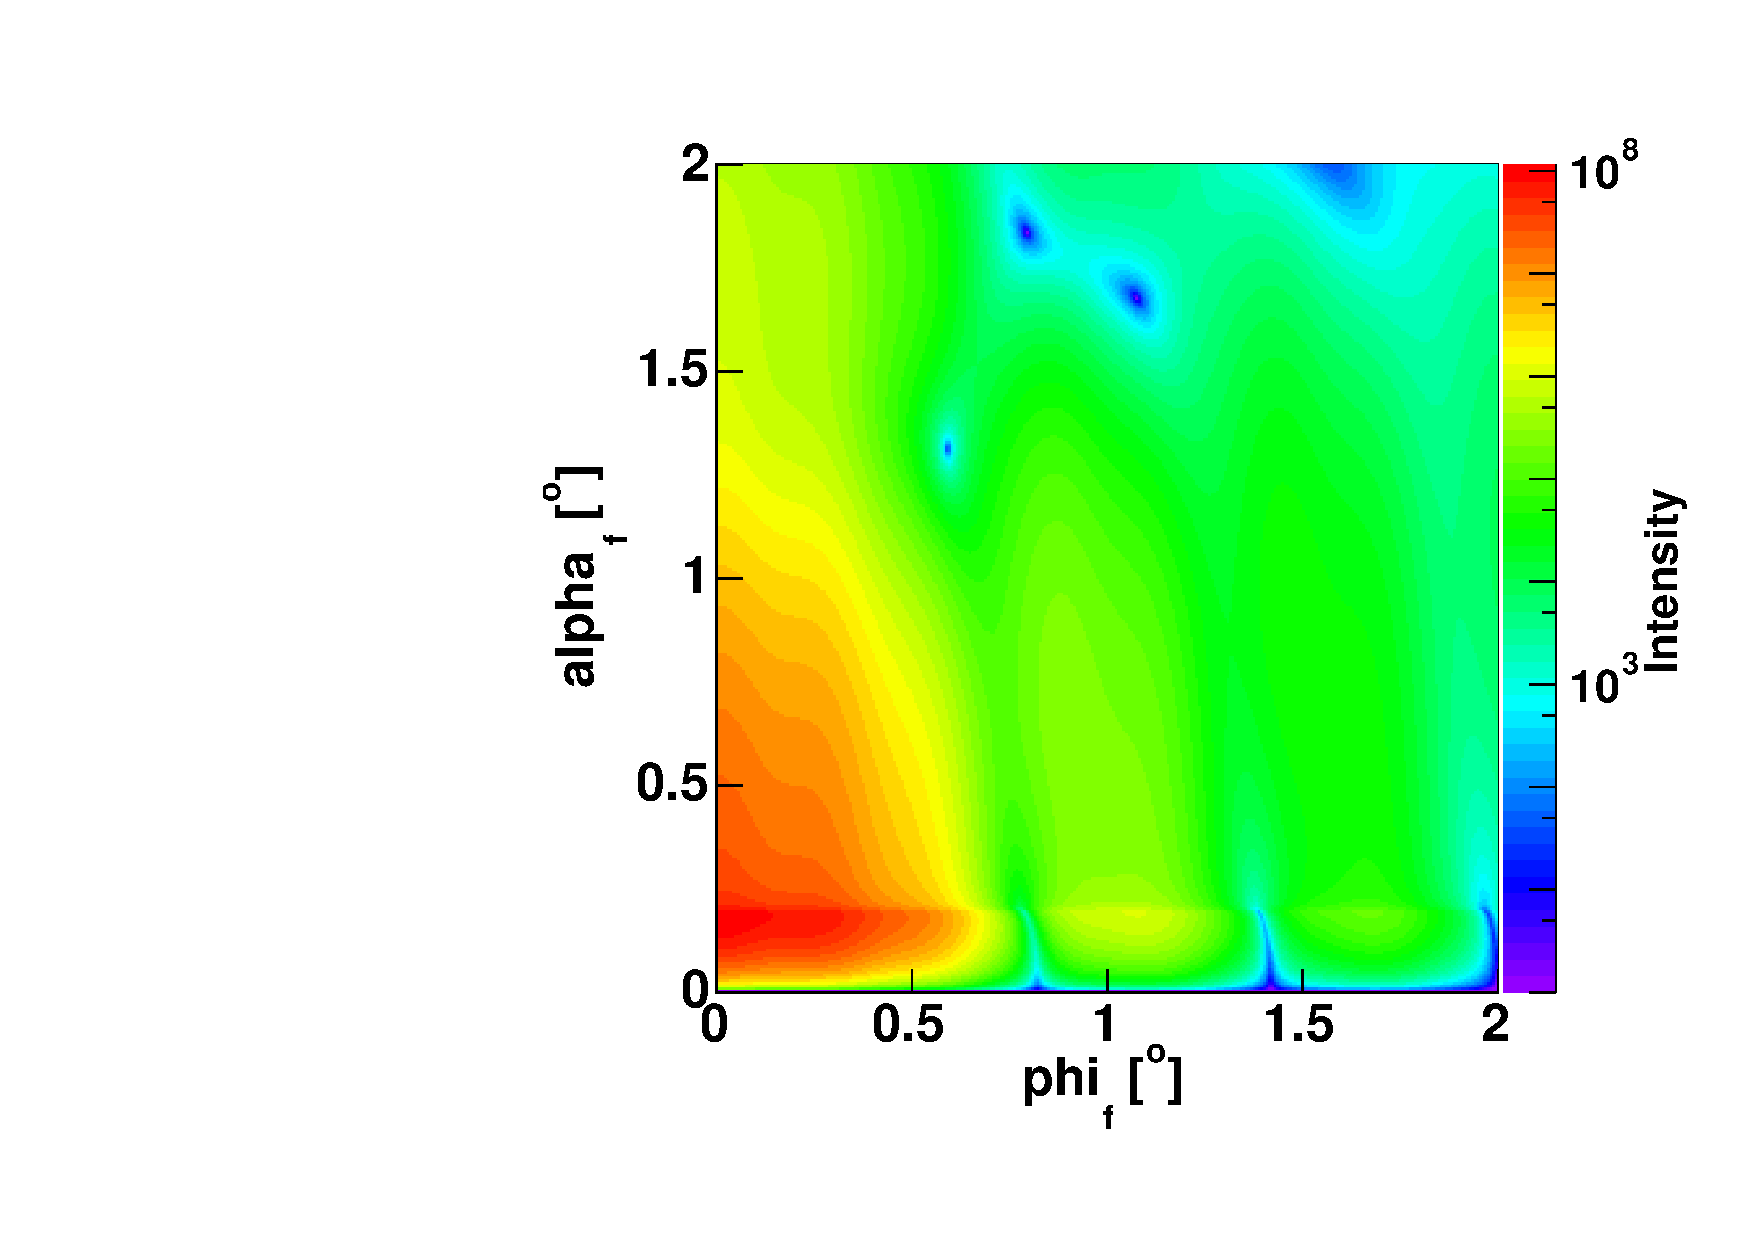
\includegraphics[width=0.5\textwidth]{Figures/HSphere_2Dlattice}
\end{center}
\caption{Output intensity scattered from a sample made of half-spheres with 2DLattice interference function. \Python\ script available at {/Examples/python/UserManual/UMInterferences2DLattice.py}.}
\label{fig:2dlatticeintensity}
\end{figure}

\FloatBarrier

\newpage{\cleardoublepage}
%%%%%%%%%%%%%%%%%%%%%%%%%%%%%%%%%%%%%%%
\subsubsection{\ding{253} \Code{InterferenceFunction2DParaCrystal(L\_1, L\_2, lattice\_angle, $\xi$, corr\_length)}} \label{paragraph2dpara}
\begin{itemize}
\item[where] $L_1$, $L_2$ are the lengths of the lattice cell,
\item[] lattice\_angle the angle between the lattice basis vectors $\mathbf{a}, \mathbf{b}$ in direct space,
\item[] $\xi$ is the angle defining the lattice orientation (set to $0$ by default).
\end{itemize}
Two predefined interference functions can be used:
\begin{itemize}
\item  \Code{createSquare(peak\_distance, corr\_length, domain\_size\_1, domain\_size\_2)}\\
where the angle between the base vectors of the lattice is set to $\pi/2$,
it creates a squared lattice,
\item \Code{createHexagonal(peak\_distance, corr\_length, domain\_size\_1, domain\_size\_2)}\\
where the angle between the base vectors of the lattice is set to $2\pi/3$ ,
\end{itemize}
where
\Code{domain\_size1, 2} are the dimensions of the paracrystal along the main axes,\\ \Code{peak\_distance} is the same in both directions and $\mathbf{a}\equiv \mathbf{x}$.\\

Probability distribution functions have to be defined. As the two-dimensional paracrystal is defined from two independent 1D paracrystals, we need two of these functions, using\\ \Code{setProbabilityDistributions(pdf\_1, pdf\_2)}, with \Code{pdf\_{1,2}} are related to each main axis of the paracrystal.

%If we use a correlation length, a prefactor of $\exp(-(L_{1,2}/corr\_length)$ is applied to the respective probability distribution. 

\paragraph{Example} The particles deposited on a substrate are half-spheres. They interference via the 2DParacrystal distribution function. The paracrystal is based on a 2D hexagonal lattice with a Gaussian probability distribution function in reciprocal space.  Script~\ref{lst:2dlatticeinterf} shows the implementation of the interference function and fig.~\ref{fig:2ddl} an example of output intensity using hemi-spherical particles The full script, UMInterferences2DParacrystal.py is available in /Examples/python/UserManual.

\begin{lstlisting}[language=python, style=eclipseboxed,numbers=none,nolol,caption={\Code{Python} script to define a "2DParacrystal" interference function between particles forming an hexagonal monolayer. },label={lst:2dlatticeinterf}]
    interference = InterferenceFunction2DParaCrystal.createHexagonal(30.0*nanometer,0.0, 40.0*micrometer, 40.0*micrometer)|
    pdf = FTDistribution2DCauchy(1.0*nanometer, 1.0*nanometer)
    interference.setProbabilityDistributions(pdf, pdf)
    particle_decoration.addInterferenceFunction(interference)
\end{lstlisting}

\begin{figure}[h]
\begin{center}
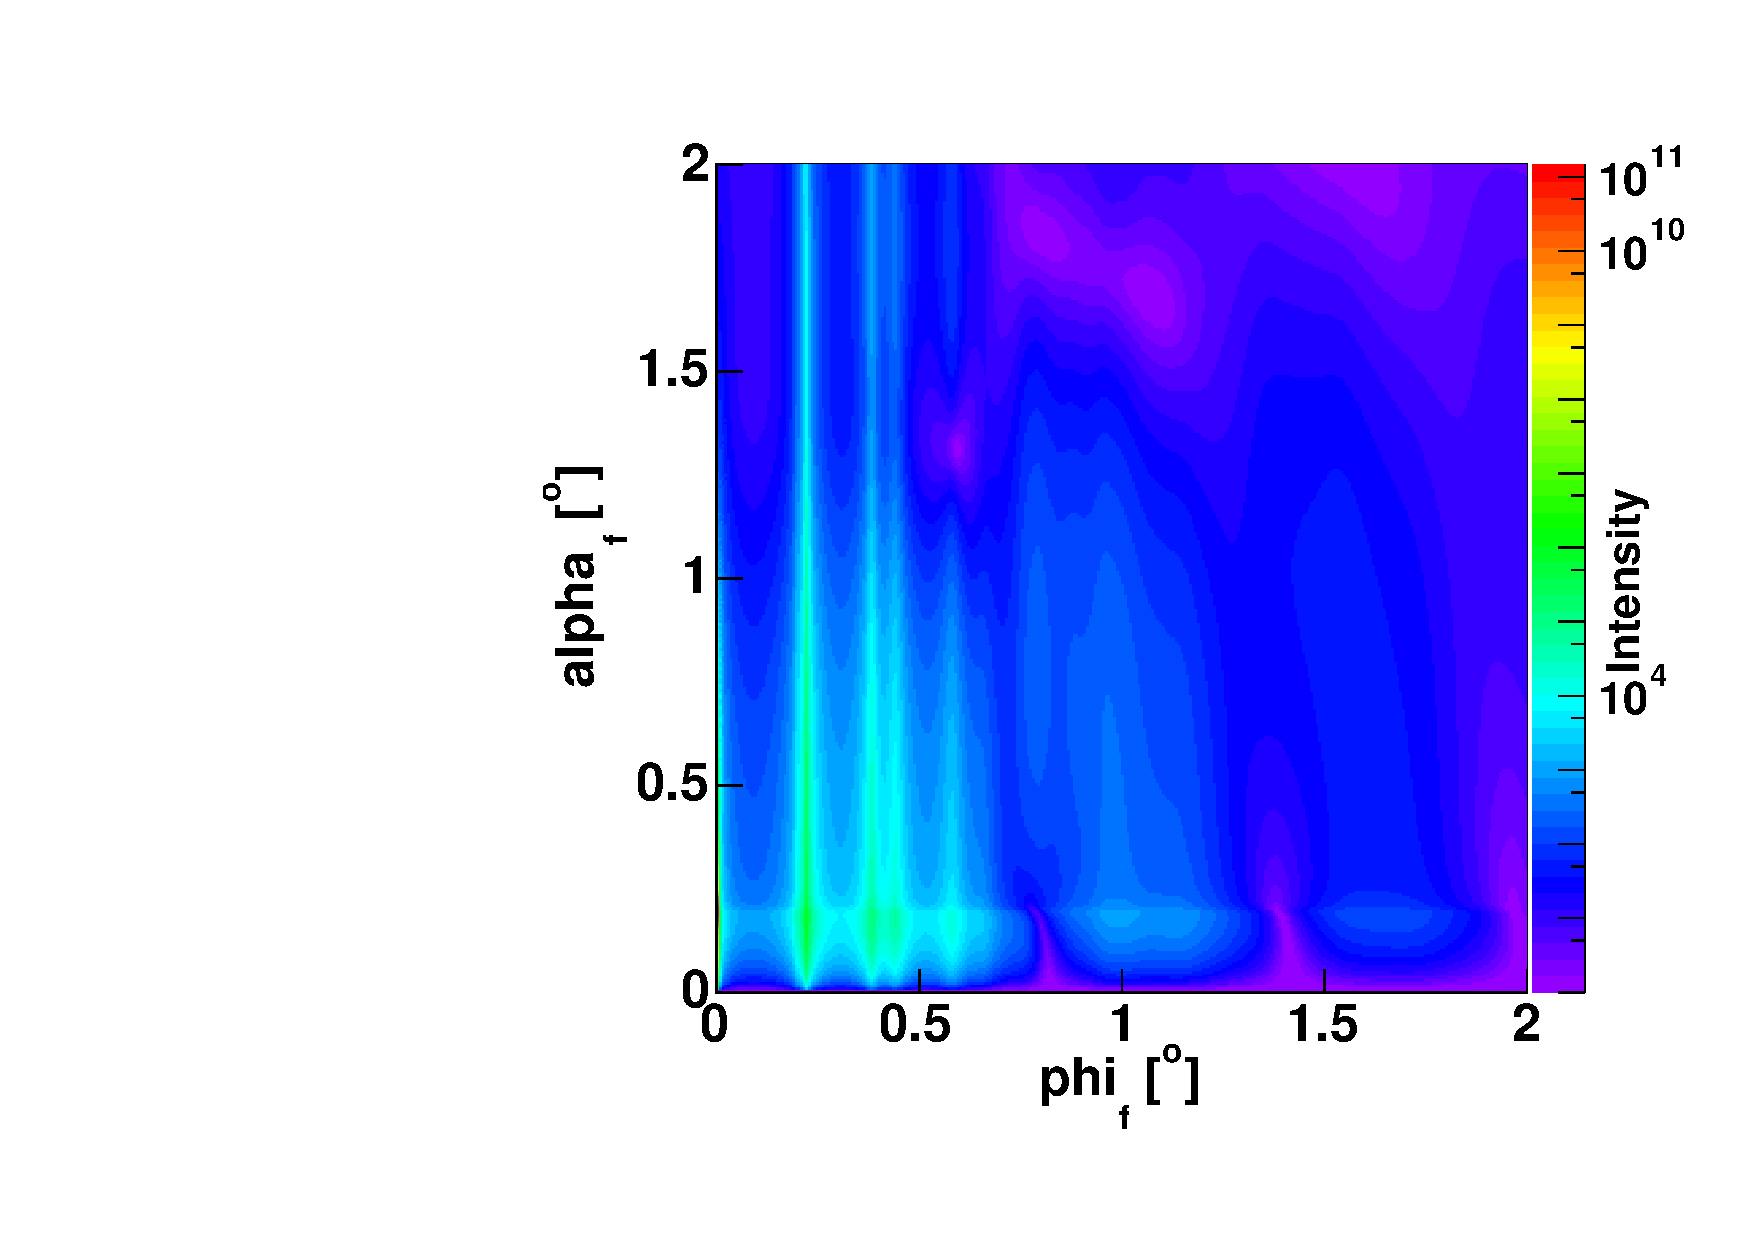
\includegraphics[width=0.5\textwidth]{Figures/HSphere_2DDL}
\end{center}
\caption{Output intensity scattered from a sample made of half-spheres with 2DParacrystal interference function.}
\label{fig:2ddl}
\end{figure}

\FloatBarrier

%%%%%%%%%%%%%%%%%%%%%%%%%%%%%%%%%%%%%%%%
\section{Summary}

\begin{landscape}
\begin{table}
\begin{tabular}{lll}
\hline
Function  & Parameters & Comments\\
\hline
\Code{InterferenceFunctionNone} \ref{paragraphnointerf} & None & disordered distribution \\
\hline
\Code{InterferenceFunction1DLattice} & \Code{lattice\_length} & use only with infinitely long/wide particles \\
 \ref{paragraph1dlatt} & $\xi=\widehat{(\mathbf{x},\mathbf{a})}$ & pdf=(Cauchy, Gauss or Voigt)  to be defined\\
\hline
 \Code{InterferenceFunction1DParaCrystal}  & peak\_distance of pdf & only Gaussian pdf implemented (no option)\\
\ref{paragraph1dpara}   & width of pdf &\\
& corr\_length (optional) & \\
\hline
 \Code{InterferenceFunction2DLattice}  & L\_1, L\_2: lattice lengths & pdf=(Cauchy, Gauss or Voigt) to be defined\\
 \ref{paragraph2dlatt}                           & lattice\_angle=$\widehat{(\mathbf{a},\mathbf{b})}$ & \\
                                                            & $\xi =\widehat{(\mathbf{x},\mathbf{a})}$ & \\                                                  
\hline
\Code{InterferenceFunction2DParaCrystal}  & L\_1, L\_2: lattice lengths & 2D pdf=(Cauchy, Gauss or Voigt) to be defined \\
\ref{paragraph2dpara}                             & lattice\_angle=$\widehat{(\mathbf{a},\mathbf{b})}$ & (1 pdf per axis) \\
& $\xi=\widehat{(\mathbf{x},\mathbf{a})}$ & \\
& corr\_length (optional) same for both axes& \\
\hline
\hline
\end{tabular}
\caption{List of interference functions implemented in \BornAgain. pdf : probability distribution function, $\mathbf{a}, \mathbf{b}$ are the lattice base vector, and $\mathbf{x}$ is the axis vector perpendicular to the detector plane.}
\end{table}
\end{landscape}
%%%%%%%%%%%%%%%%%%%%%%%%%%%%%%
